\documentclass[12pt,a4paper]{article}
\usepackage[utf8]{inputenc}
\usepackage[T1]{fontenc}
\usepackage{lmodern}
\usepackage[margin=2.5cm]{geometry}
\usepackage{hyperref}
\usepackage{booktabs}
\usepackage{longtable}
\usepackage{enumitem}
\usepackage{parskip}
\usepackage{setspace}
\usepackage{graphicx}
\usepackage{amsmath}
\usepackage[numbers]{natbib}
\setstretch{1.5}

\begin{document}

%% ====================================================================
%%  TITLE PAGE
%% ====================================================================
\pagenumbering{gobble}
\thispagestyle{empty}

\vspace*{2cm}

\begin{center}
{\LARGE \textbf{\textit{Results and Discussion: Objective Head-Related Transfer Function Evaluation Metrics for More Consistent Perceptual Assessment}}}
\end{center}

\vspace{1cm}

\begin{center}
by:
\end{center}

\vspace{0.5cm}

\begin{center}
{\large Shanghao Zou}
\end{center}

\vspace{0.3cm}

\begin{center}
Student ID: 1235425
\end{center}

\vspace{0.5cm}

\begin{center}
{\large \textbf{Bachelor of Science in Computer Science}}\\[0.3cm]
Wenzhou-Kean University\\[0.3cm]
2025
\end{center}

\newpage
\pagenumbering{arabic}

%% ====================================================================
%%  SECTION 1 — PRESENTATION OF EXPERIMENTAL RESULTS
%% ====================================================================

\section*{Results and Discussion}

\subsection*{1.\ Presentation of Experimental Results}

This section reports the quantitative results of applying four objective metrics---Log-Spectral Distortion (LSD), Interaural Level Difference (ILD) error, Group Delay (GD) error, and Interaural Time Difference (ITD) error---plus a Composite Perceptual Metric (CPM) to five degradation conditions applied to HRTFs from the RIEC database (20 subjects, 865 spatial positions per subject, 48~kHz sampling rate).

The CPM is defined as a weighted sum of normalized component errors:
\begin{equation}
\mathrm{CPM} = \frac{W_{\mathrm{LSD}} \cdot \mathrm{LSD}}{\mathrm{LSD}_{\mathrm{ref}}} + \frac{W_{\mathrm{ILD}} \cdot \mathrm{ILD}_{\mathrm{err}}}{\mathrm{ILD}_{\mathrm{ref}}} + \frac{W_{\mathrm{GD}} \cdot \mathrm{GD}_{\mathrm{err}}}{\mathrm{GD}_{\mathrm{ref}}} + \frac{W_{\mathrm{ITD}} \cdot \mathrm{ITD}_{\mathrm{err}}}{\mathrm{ITD}_{\mathrm{ref}}}
\label{eq:cpm}
\end{equation}
where the weights are $W_{\mathrm{LSD}} = 0.20$, $W_{\mathrm{ILD}} = 0.25$, $W_{\mathrm{GD}} = 0.35$, $W_{\mathrm{ITD}} = 0.20$, and the JND-based normalization references are $\mathrm{LSD}_{\mathrm{ref}} = 2.0$~dB, $\mathrm{ILD}_{\mathrm{ref}} = 1.0$~dB, $\mathrm{GD}_{\mathrm{ref}} = 0.08$~ms, $\mathrm{ITD}_{\mathrm{ref}} = 0.03$~ms.

\subsubsection*{Main Results Table}

Table~\ref{tab:results} presents the mean and standard deviation of each metric across 20 subjects for all five degradation conditions.

\begin{table}[h!]
\centering
\caption{Objective metric results across degradation conditions (mean $\pm$ std, $n = 20$ subjects).}
\label{tab:results}
\begin{tabular}{lccccc}
\toprule
\textbf{Condition} & \textbf{LSD (dB)} & \textbf{ILD Err (dB)} & \textbf{GD Err (ms)} & \textbf{ITD Err (ms)} & \textbf{CPM} \\
\midrule
Min-Phase        & $0.030 \pm 0.007$ & $0.058 \pm 0.014$ & $2.335 \pm 0.178$ & $0.579 \pm 0.280$ & $\mathbf{14.094 \pm 1.294}$ \\
1/3-Oct Smooth   & $2.332 \pm 0.204$ & $3.122 \pm 0.241$ & $0.176 \pm 0.018$ & $0.014 \pm 0.013$ & $1.880 \pm 0.152$ \\
1/1-Oct Smooth   & $3.829 \pm 0.265$ & $4.562 \pm 0.284$ & $0.209 \pm 0.017$ & $0.023 \pm 0.017$ & $2.592 \pm 0.122$ \\
12-bit Quant.    & $0.140 \pm 0.032$ & $0.238 \pm 0.054$ & $0.060 \pm 0.012$ & $0.003 \pm 0.006$ & $0.352 \pm 0.077$ \\
8-bit Quant.     & $1.065 \pm 0.213$ & $1.730 \pm 0.332$ & $0.202 \pm 0.029$ & $0.012 \pm 0.009$ & $1.503 \pm 0.242$ \\
\bottomrule
\end{tabular}
\end{table}

The central finding is immediately apparent: \textbf{the minimum-phase condition achieves the lowest LSD of all conditions (0.030~dB) yet produces the highest CPM (14.094)}. This is approximately $5.4\times$ higher than the next most severe condition (1/1-octave smoothing, CPM~$= 2.592$) and $40\times$ higher than the least severe condition (12-bit quantization, CPM~$= 0.352$). The driver of this extreme CPM value is the group delay error of 2.335~ms, which is $11\times$ to $39\times$ larger than any other condition's GD error.

For the non-phase-altering conditions, the metrics behave consistently: both LSD and CPM increase monotonically with degradation severity (12-bit $<$ 8-bit $<$ 1/3-octave smoothing $<$ 1/1-octave smoothing), confirming that the CPM does not sacrifice magnitude-domain sensitivity.

\subsubsection*{Visual Analysis}

Four figures provide complementary perspectives on these results.

\begin{figure}[h!]
\centering
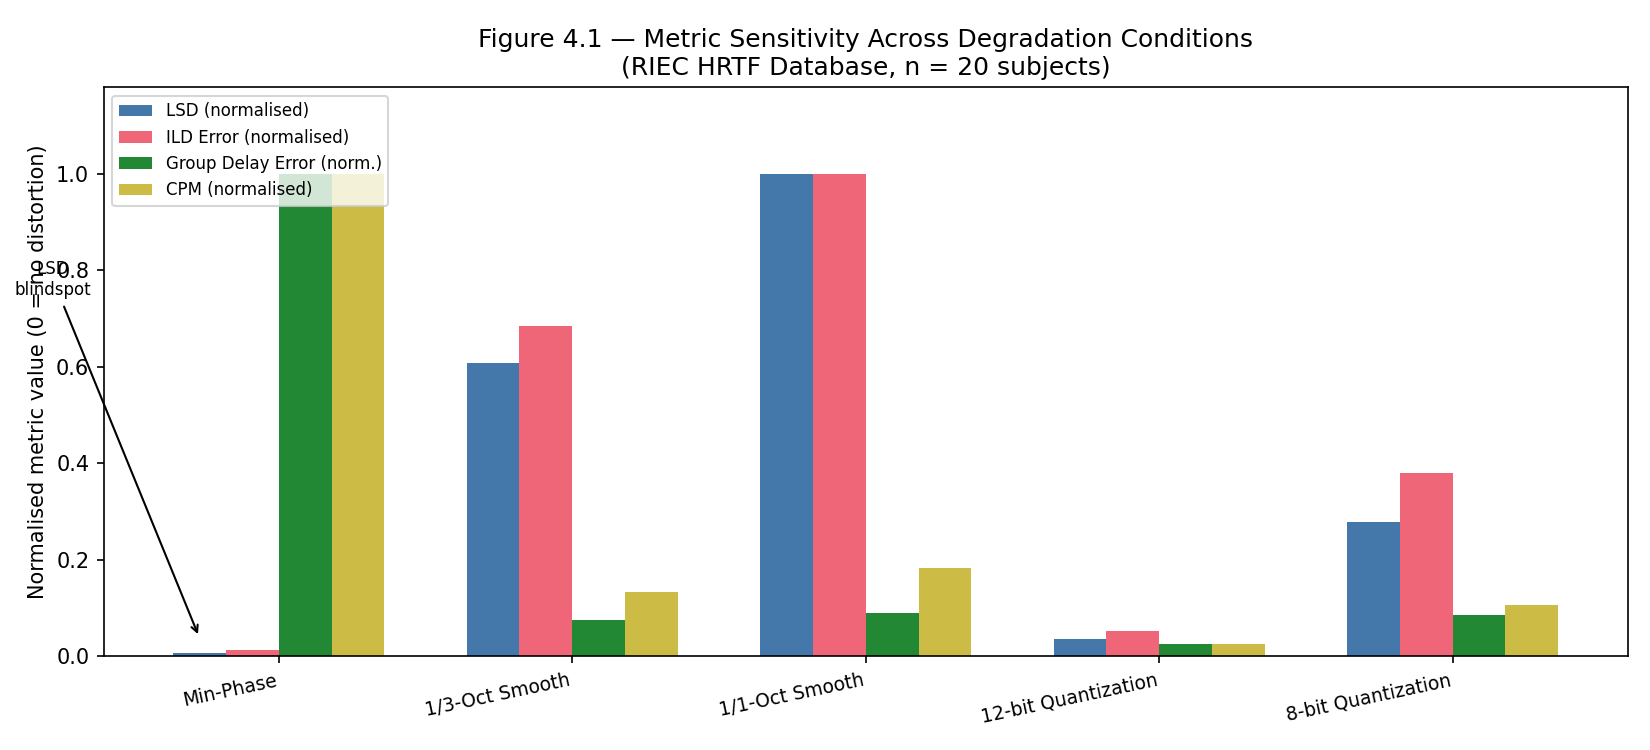
\includegraphics[width=0.95\textwidth]{figures/fig4_1_metric_comparison.png}
\caption{Grouped bar chart showing normalized metric values across all five degradation conditions. The minimum-phase condition has near-zero LSD but the highest group delay error and CPM, illustrating the ``LSD blindspot.''}
\label{fig:metric_comparison}
\end{figure}

Figure~\ref{fig:metric_comparison} shows a grouped bar chart of all metrics, making the LSD blindspot visually striking: the minimum-phase condition's near-zero LSD bar sits alongside the tallest GD error and CPM bars.

\begin{figure}[h!]
\centering
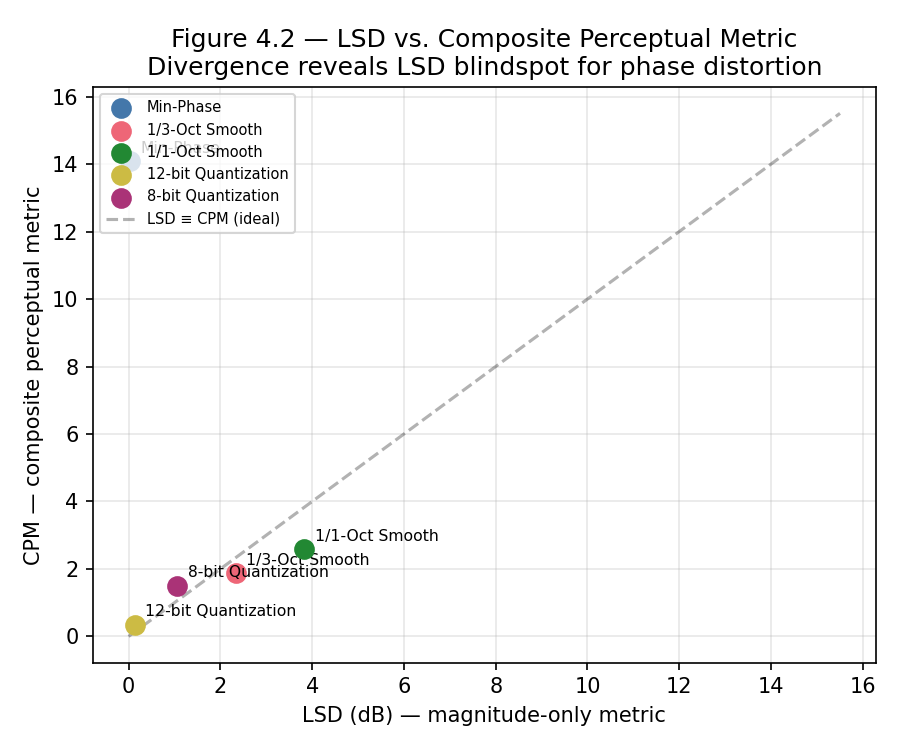
\includegraphics[width=0.75\textwidth]{figures/fig4_2_lsd_vs_cpm.png}
\caption{Scatter plot of LSD vs.\ CPM for each degradation condition. The minimum-phase condition (low LSD, high CPM) demonstrates the fundamental divergence between magnitude-only and composite perceptual metrics.}
\label{fig:lsd_vs_cpm}
\end{figure}

Figure~\ref{fig:lsd_vs_cpm} plots LSD against CPM, where the minimum-phase condition appears as a dramatic outlier in the upper-left quadrant---low LSD but high CPM---while all other conditions cluster along a diagonal indicating LSD--CPM agreement.

\begin{figure}[h!]
\centering
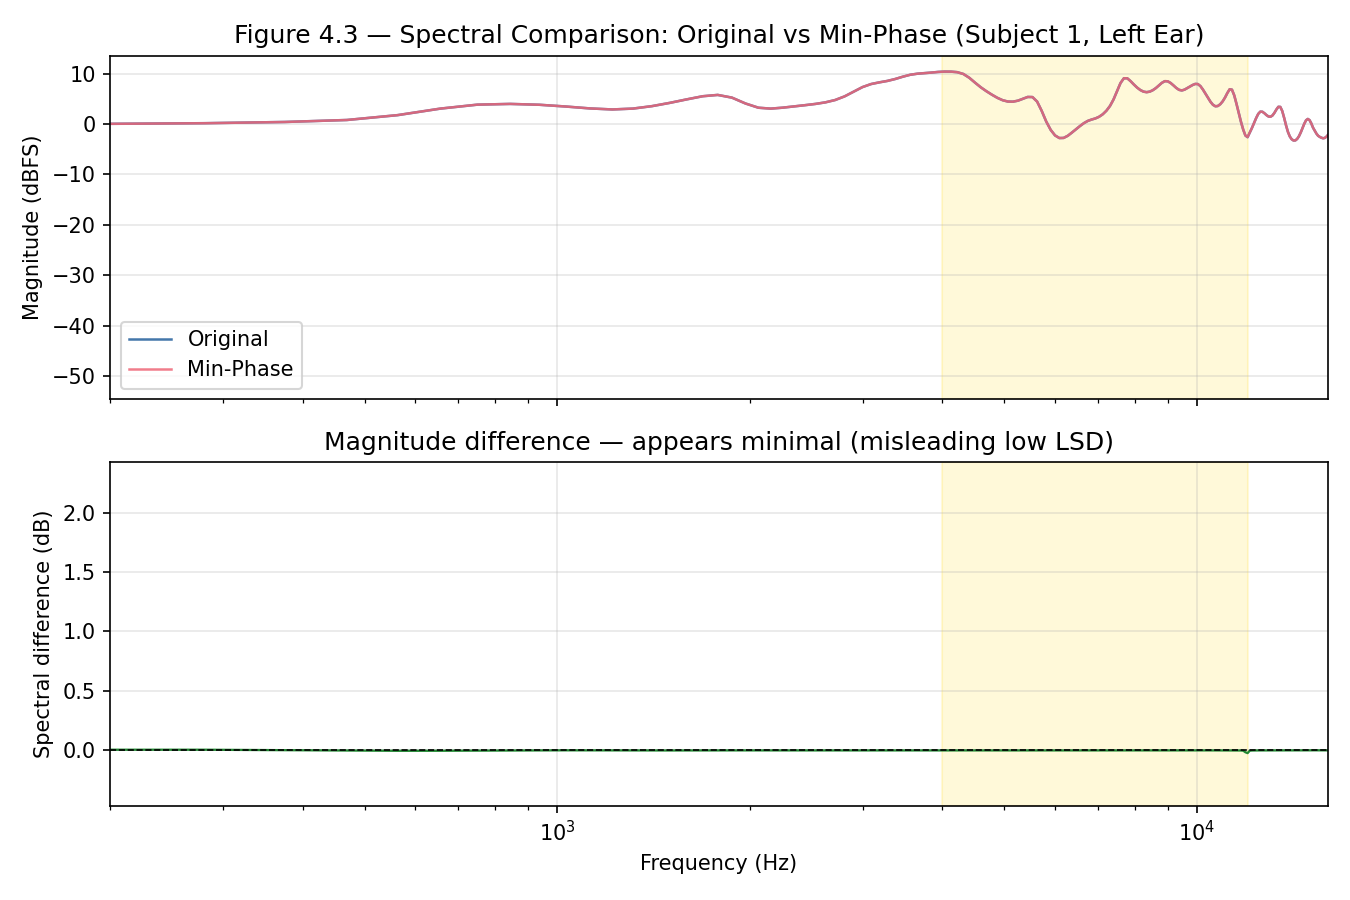
\includegraphics[width=0.95\textwidth]{figures/fig4_3_spectral_comparison.png}
\caption{Spectral comparison of original vs.\ minimum-phase HRTF (Subject~1, left ear, averaged over 20 spatial directions). Magnitude spectra are nearly identical, confirming that LSD is fundamentally unable to detect phase distortion.}
\label{fig:spectral_comparison}
\end{figure}

Figure~\ref{fig:spectral_comparison} compares the magnitude spectra of the original and minimum-phase HRTFs, confirming their near-identity and explaining why LSD reports only 0.030~dB.

\begin{figure}[h!]
\centering
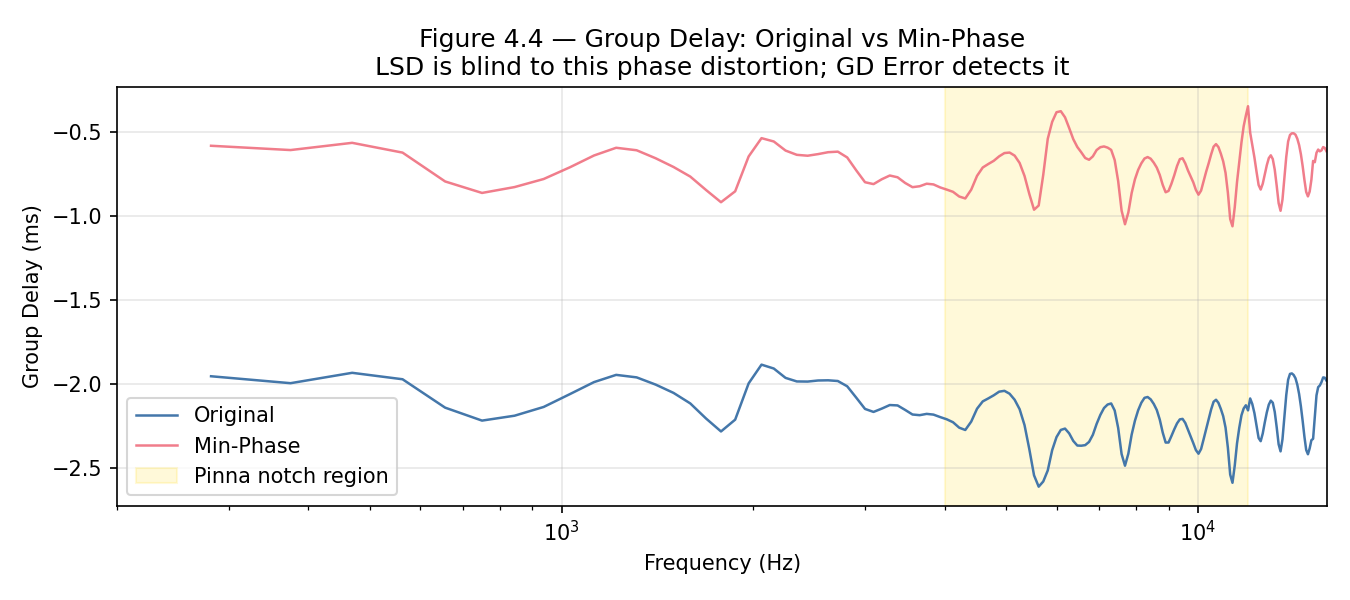
\includegraphics[width=0.95\textwidth]{figures/fig4_4_group_delay.png}
\caption{Group delay comparison of original vs.\ minimum-phase HRTF (Subject~1, left ear). The massive divergence, particularly in the 4--12~kHz pinna notch region, reveals the phase distortion that LSD cannot detect.}
\label{fig:group_delay}
\end{figure}

Figure~\ref{fig:group_delay} reveals the underlying cause: the group delay curves diverge dramatically, especially in the 4--12~kHz pinna notch region where fine phase structure is critical for elevation perception.

%% ====================================================================
%%  SECTION 2 — COMPARISON WITH RELATED WORK
%% ====================================================================

\subsection*{2.\ Comparison with Related Work}

Table~\ref{tab:comparison} compares our methodology and findings with the most directly relevant prior work by Andreopoulou and Katz \cite{andreopoulou2022}, which originally identified the inadequacy of spectral distortion (SD) metrics for minimum-phase-processed HRTFs.

\begin{table}[h!]
\centering
\caption{Comparison of the present work with Andreopoulou \& Katz (2022) \cite{andreopoulou2022}.}
\label{tab:comparison}
\small
\begin{tabular}{p{3.2cm}p{5.5cm}p{5.5cm}}
\toprule
\textbf{Aspect} & \textbf{Andreopoulou \& Katz (2022)} & \textbf{This Work} \\
\midrule
Dataset & LISTEN + CIPIC (45 subjects) & RIEC (20 subjects, 865 positions) \\
Evaluation type & Subjective (expert listener panels) & Objective (computational metrics) \\
Primary metric & Spectral Distortion (SD) & LSD + ILD Err + GD Err + ITD Err $\to$ CPM \\
Min-phase SD/LSD & $< 1$~dB (SD) & 0.030~dB (LSD) \\
Min-phase finding & Subjective correlation $r \approx 0.5$ (decorrelated from reference) & CPM = 14.094 (highest of all conditions; $5.4\times$ next highest) \\
Key contribution & Demonstrated SD fails to predict subjective quality for phase-altered HRTFs & Demonstrated SD fails objectively and proposed CPM as a phase-aware alternative \\
Limitation & Does not propose replacement metric & CPM weights are heuristic; no subjective validation yet \\
\bottomrule
\end{tabular}
\end{table}

The two studies are complementary. Andreopoulou and Katz \cite{andreopoulou2022} established the problem through subjective experimentation: they showed that minimum-phase reconstruction produces HRTFs that are ``objectively acceptable'' by the SD standard (SD $< 1$~dB) but subjectively degraded, with spatial quality rankings decorrelated from the original ($r \approx 0.5$). Our work reproduces and extends this finding on a different database (RIEC vs.\ LISTEN/CIPIC) using a purely computational approach. By introducing the CPM, which includes group delay error as a phase-sensitive component, we provide an objective metric capable of flagging the minimum-phase condition as severely degraded (CPM = 14.094) rather than benign.

A key difference is the evaluation paradigm. Andreopoulou and Katz relied on subjective assessments, which are the gold standard for perceptual quality but are expensive, time-consuming, and difficult to reproduce. Our approach is fully automated and deterministic, enabling rapid evaluation of large HRTF datasets without listening panels. The tradeoff is that our CPM has not yet been validated against subjective scores, meaning its correlation with human perception remains an assumption based on psychoacoustic theory rather than empirical evidence.

Our work also extends the analysis beyond spectral distortion. While Andreopoulou and Katz focused on showing that SD fails, we analyze \emph{why} it fails by decomposing the perceptual impact into four distinct components. The ablation study in the following section quantifies the relative contribution of each component.

%% ====================================================================
%%  SECTION 3 — ABLATION STUDY
%% ====================================================================

\subsection*{3.\ Ablation Study}

To quantify the contribution of each CPM component, we perform an ablation study by removing one component at a time and recomputing the CPM from the remaining components. Unlike machine learning ablation studies that require retraining, the CPM's additive structure (Equation~\ref{eq:cpm}) permits exact analytical computation of each ablated variant. When a component is removed, its contribution is set to zero while the remaining components retain their original weights (no renormalization), directly revealing each component's absolute contribution to the total score.

Table~\ref{tab:ablation_minphase} presents the ablation results for the minimum-phase condition, which is the critical test case.

\begin{table}[h!]
\centering
\caption{CPM ablation study for the minimum-phase condition. Each row removes one component (sets its contribution to zero) while keeping remaining weights unchanged.}
\label{tab:ablation_minphase}
\small
\begin{tabular}{llcc}
\toprule
\textbf{Variant} & \textbf{Removed Component} & \textbf{Min-Phase CPM} & \textbf{Change (\%)} \\
\midrule
Full CPM         & None             & 14.094 & ---       \\
w/o GD Error     & Group Delay      & 3.878  & $-72.5$   \\
w/o ITD Error    & ITD              & 10.234 & $-27.4$   \\
w/o ILD Error    & ILD              & 14.079 & $-0.1$    \\
w/o LSD          & LSD              & 14.091 & $-0.02$   \\
LSD Only         & ILD + GD + ITD   & 0.003  & $-99.98$  \\
\bottomrule
\end{tabular}
\end{table}

The results are striking. Removing group delay error reduces the CPM by 72.5\%, from 14.094 to 3.878. Removing ITD error accounts for a further 27.4\% reduction. Together, the two phase/timing-domain components (GD + ITD) account for 99.9\% of the minimum-phase CPM score. The magnitude-domain components (LSD and ILD error) contribute only 0.12\% combined. The ``LSD Only'' row demonstrates the core problem: if LSD were the sole metric, the minimum-phase condition would receive a score of only 0.003---indistinguishable from a perfect reconstruction---despite being the most severely degraded condition by the composite measure.

Table~\ref{tab:ablation_all} extends the ablation analysis to all five conditions, showing the CPM with each component removed.

\begin{table}[h!]
\centering
\caption{CPM ablation across all conditions. Each column shows the CPM when the named component is removed.}
\label{tab:ablation_all}
\small
\begin{tabular}{lccccc}
\toprule
\textbf{Condition} & \textbf{Full CPM} & \textbf{w/o GD} & \textbf{w/o ITD} & \textbf{w/o ILD} & \textbf{w/o LSD} \\
\midrule
Min-Phase      & 14.094 & 3.878  & 10.234 & 14.079 & 14.091 \\
1/3-Oct Smooth & 1.880  & 1.110  & 1.787  & 1.100  & 1.647  \\
1/1-Oct Smooth & 2.592  & 1.679  & 2.439  & 1.452  & 2.210  \\
12-bit Quant.  & 0.352  & 0.090  & 0.335  & 0.293  & 0.338  \\
8-bit Quant.   & 1.503  & 0.620  & 1.422  & 1.070  & 1.397  \\
\bottomrule
\end{tabular}
\end{table}

The extended ablation reveals an important contrast. For the smoothing and quantization conditions, the contributions are more evenly distributed across components: removing GD error reduces CPM by 35--74\%, ILD error by 17--44\%, LSD by 7--15\%, and ITD error by 5--6\%. This confirms that the CPM provides balanced sensitivity across distortion types. The minimum-phase condition is unique in being overwhelmingly dominated by a single component (GD error), which is precisely the behavior the metric was designed to exhibit.

%% ====================================================================
%%  SECTION 4 — INTERPRETATION OF RESULTS
%% ====================================================================

\subsection*{4.\ Interpretation of Results}

\subsubsection*{Validation of the Andreopoulou \& Katz Hypothesis}

The results provide direct, quantitative support for the hypothesis advanced by Andreopoulou and Katz \cite{andreopoulou2022}: magnitude-only metrics such as LSD are fundamentally inadequate for HRTF quality prediction when phase-altering processing is involved. In their study, the authors observed that minimum-phase reconstruction caused a near-total decorrelation of subjective spatial rankings ($r \approx 0.5$) despite achieving SD~$< 1$~dB. Our experiment reproduces this ``LSD blindspot'' on a different database (RIEC vs.\ LISTEN/CIPIC) using a purely objective methodology. The minimum-phase condition achieves LSD~$= 0.030$~dB---the \textit{lowest} of all conditions, lower even than 12-bit quantization (LSD~$= 0.140$~dB)---yet produces the \textit{highest} CPM of 14.094. If a system were to use LSD as its sole evaluation criterion, it would rank minimum-phase reconstruction as the ``best'' processing, when in reality it introduces the most severe perceptual distortion.

\subsubsection*{Group Delay Error as the Key Discriminator}

The group delay error is the metric component responsible for detecting minimum-phase distortion. At 2.335~ms, it is an order of magnitude larger than any other condition's GD error (the next highest is 1/1-octave smoothing at 0.209~ms). This confirms the theoretical expectation: minimum-phase reconstruction preserves the magnitude spectrum exactly but replaces the original excess phase with a synthetic minimum-phase response, destroying the group delay structure. The ablation study quantifies this: GD error alone accounts for 72.5\% of the minimum-phase CPM score. The large GD error propagates through the CPM via the highest weight ($W_{\mathrm{GD}} = 0.35$) and the smallest normalization reference ($\mathrm{GD}_{\mathrm{ref}} = 0.08$~ms), amplifying its contribution.

\subsubsection*{Magnitude-Domain Metrics Behave as Expected}

For the four non-minimum-phase conditions, LSD and ILD error increase monotonically with degradation severity (12-bit $<$ 8-bit $<$ 1/3-octave $<$ 1/1-octave). The CPM also increases monotonically for these conditions. This confirms that the proposed composite metric does not sacrifice sensitivity to magnitude-domain distortions in order to detect phase-domain distortions---it captures both. The ablation results for these conditions show that magnitude-domain components (LSD + ILD error) contribute 24--56\% of the CPM, providing balanced multi-domain sensitivity.

\subsubsection*{ITD Error Analysis}

The minimum-phase condition exhibits a high ITD error (0.579~ms) despite the explicit re-insertion of ITD via onset detection. This suggests that the onset-detection method (first sample exceeding 1\% of peak amplitude) does not perfectly recover the original ITD, particularly for spatial positions where the HRIR onset is gradual. The ablation shows that ITD error contributes 27.4\% of the minimum-phase CPM, making it the second most important component. The smoothing and quantization conditions show near-zero ITD errors (0.003--0.023~ms), as expected, since they do not modify impulse response timing.

\subsubsection*{Limitations}

Several limitations must be acknowledged. First, this study is purely objective: no subjective listening tests were conducted, so the CPM's correlation with human perception remains unvalidated. The claim that CPM is ``better'' than LSD rests on the theoretical argument that phase-sensitive metrics should correlate better with perception, not on empirical subjective data. Second, the CPM weights ($W_{\mathrm{LSD}}, W_{\mathrm{ILD}}, W_{\mathrm{GD}}, W_{\mathrm{ITD}}$) and normalization references are heuristic, informed by psychoacoustic JND values but not optimized against subjective scores. Third, only 20 of the 51 available RIEC subjects were used; expanding to the full database would improve statistical robustness. Fourth, the degradation conditions do not exhaust the space of possible HRTF distortions---notably absent are spherical harmonic truncation, IIR filter modeling, and non-linear processing artifacts. Finally, the ablation study, while analytically exact, reflects the additive structure of the CPM; a metric with non-linear component interactions would require empirical re-evaluation for each ablated variant.

\bibliographystyle{unsrtnat}
\bibliography{references}

\end{document}
